\documentclass{beamer}

% Package imports
\usepackage{amsmath}
\usepackage{listings}
\usepackage{xcolor}
\usepackage{graphicx}

% Define custom Star Trek DS9 colors
\definecolor{ds9blue}{RGB}{25,25,112}
\definecolor{ds9gold}{RGB}{218,165,32}
\definecolor{ds9grey}{RGB}{105,105,105}
\definecolor{ds9red}{RGB}{178,34,34}

% Setup theme with custom colors
\usetheme{Madrid}
\usecolortheme{default}

% Color customizations
\setbeamercolor{palette primary}{bg=ds9blue,fg=white}
\setbeamercolor{palette secondary}{bg=ds9grey,fg=white}
\setbeamercolor{palette tertiary}{bg=ds9gold,fg=black}
\setbeamercolor{palette quaternary}{bg=ds9red,fg=white}
\setbeamercolor{structure}{fg=ds9blue}
\setbeamercolor{title}{fg=ds9gold}
\setbeamercolor{subtitle}{fg=ds9gold}
\setbeamercolor{frametitle}{bg=ds9blue,fg=white}
\setbeamercolor{block title}{bg=ds9blue,fg=white}
\setbeamercolor{block body}{bg=ds9grey!20,fg=black}

% Configure code listings
\lstset{
  language=C++,
  basicstyle=\ttfamily\small,
  keywordstyle=\color{ds9blue}\bfseries,
  stringstyle=\color{ds9red},
  commentstyle=\color{ds9grey}\itshape,
  numbers=left,
  numberstyle=\tiny\color{ds9grey},
  breaklines=true,
  showstringspaces=false,
  frame=single,
  rulecolor=\color{ds9blue}
}

% Title page configuration
\title[Caesar Cipher]{CS12: Caesar Cipher Encryption}
\subtitle{Understanding Cryptography Basics with C++}
\author[Mr. Gullo]{Mr. Gullo}
\date[March 2025]{March, 2025}
\institute{Computer Science Department}

\begin{document}

\begin{frame}
    \titlepage
\end{frame}

\begin{frame}
    \frametitle{Table of Contents}
    \tableofcontents
\end{frame}

\section{Introduction to Cryptography}

\begin{frame}
    \frametitle{Learning Objectives}
    By the end of this lesson, you will be able to:
    \begin{itemize}
        \item Understand the basic principles of cryptography
        \item Explain how the Caesar cipher works
        \item Implement Caesar cipher encryption and decryption in C++
        \item Calculate encryption and decryption keys
        \item Apply modular arithmetic in cryptographic algorithms
    \end{itemize}
\end{frame}

\begin{frame}
    \frametitle{What is Cryptography?}
    \begin{columns}
    \column{0.6\textwidth}
    \begin{itemize}
        \item The practice of secure communication in the presence of adversaries
        \item From Greek: "kryptós" (hidden) and "graphein" (to write)
        \item Historically used for military and diplomatic communications
        \item Now essential for internet security, banking, and privacy
    \end{itemize}
    
    \column{0.4\textwidth}
    \begin{figure}
        \centering
        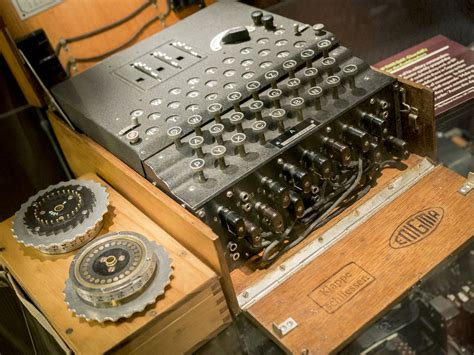
\includegraphics[width=0.8\linewidth]{th-1232469891.jpg}
    \end{figure}
    \end{columns}
    
    \begin{block}{Key Terms}
        \begin{itemize}
            \item \textbf{Plaintext}: Original, readable message
            \item \textbf{Encryption}: Process of converting plaintext to ciphertext
            \item \textbf{Ciphertext}: Encrypted, unreadable message
            \item \textbf{Decryption}: Process of converting ciphertext back to plaintext
            \item \textbf{Key}: Secret information used in encryption/decryption
        \end{itemize}
    \end{block}
\end{frame}

\section{The Caesar Cipher}

\begin{frame}
    \frametitle{What is the Caesar Cipher?}
    \begin{itemize}
        \item One of the earliest and simplest encryption techniques
        \item Named after Julius Caesar, who used it to communicate with his generals
        \item A type of \textbf{substitution cipher}
        \item Each letter in the plaintext is shifted a certain number of places down the alphabet
        \item Example: With a shift of 3, 'A' becomes 'D', 'B' becomes 'E', etc.
    \end{itemize}
    
    \begin{alertblock}{Historical Note}
        Caesar reportedly used a shift of 3 for all his communications, making it quite easy to break if you knew the system!
    \end{alertblock}
\end{frame}

\begin{frame}
    \frametitle{How Caesar Cipher Works}
    \begin{columns}
    \column{0.55\textwidth}
    \textbf{Encryption:}
    \begin{itemize}
        \item Each letter is shifted forward by a fixed value (the key)
        \item If shift goes past 'z', it wraps around to 'a'
    \end{itemize}
    
    \textbf{Example with key = 3:}
    \begin{itemize}
        \item a → d
        \item b → e
        \item c → f
        \item z → c
    \end{itemize}
    
    \column{0.45\textwidth}
    \begin{figure}
        \centering
        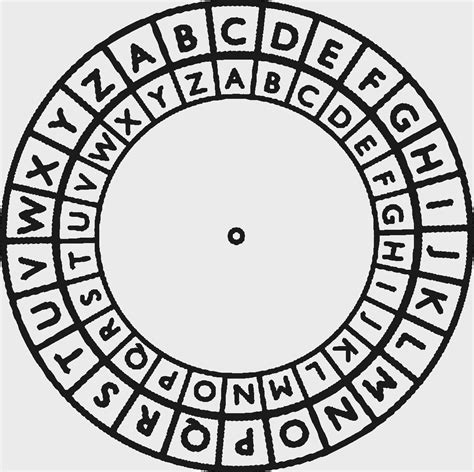
\includegraphics[width=0.75\linewidth]{th-3125735322.jpg}
    \end{figure}
    \end{columns}
    
    \begin{block}{Mathematical Representation}
        For a key $K$, each letter $L$ becomes:
        $E(L) = (L + K) \mod 26$
        
        Where letters are represented by their position in the alphabet (a=0, b=1, ..., z=25)
    \end{block}
\end{frame}

\begin{frame}
    \frametitle{Decryption in Caesar Cipher}
    \begin{itemize}
        \item Decryption is the reverse process of encryption
        \item Each letter is shifted backward by the same fixed value
        \item If shift goes past 'a', it wraps around to 'z'
    \end{itemize}
    
    \begin{block}{Mathematical Representation}
        For a key $K$, decryption of letter $C$ is:
        $D(C) = (C - K) \mod 26$
        
        \textbf{Alternatively}, we can use a "decryption key":
        $D_K = 26 - K \mod 26$
        
        Then decrypt using: $D(C) = (C + D_K) \mod 26$
    \end{block}
    
    \textbf{Example:} If encryption key is 3, decryption key is $26 - 3 = 23$
\end{frame}

\section{Implementation in C++}

\begin{frame}[fragile]
    \frametitle{caesarSingle.cpp - Overview}
    
    Let's examine the complete program:
    
    \begin{lstlisting}
char caesarShift(char message, char key){
    return 'a' + (message - 'a' + key - 'a') % 26;}

char getDecodeKey(char key){
    return 'a' + (26 - key + 'a') % 26;}
int main(){
    char plainText, key, secretMessage, decodeKey, decodedMessage;
    cout << "Plain text: ";
    cin >> plainText;
    cout << "Key: ";
    cin >> key;
    secretMessage = caesarShift(plainText, key);
    decodeKey = getDecodeKey(key);
    decodedMessage = caesarShift(secretMessage, decodeKey);
    cout << "Secret Message: " << secretMessage << endl;
    cout << "Decode key: " << decodeKey << endl;
    cout << "Decoded Message: " << decodedMessage << endl;
    return 0;
}
    \end{lstlisting}
\end{frame}

\begin{frame}[fragile]
    \frametitle{Program Output}
    
    When we run the program with inputs 'a' and 'x', we get:
    
    \begin{lstlisting}[language={}]
Plain text: a
Key: x
Secret Message: x
Decode key: d
Decoded Message: a
    \end{lstlisting}
    
    \begin{itemize}
        \item Input 'a' was encrypted to 'x' using key 'x'
        \item Decode key was calculated as 'd'
        \item 'x' was decrypted back to 'a' using the decode key 'd'
        \item The original message was successfully recovered!
    \end{itemize}
\end{frame}

\section{Extending the Caesar Cipher}

\begin{frame}[fragile]
    \frametitle{Limitations of Current Implementation}
    
    Our current implementation has several limitations:
    
    \begin{itemize}
        \item Only handles single characters, not strings
        \item Only works with lowercase letters
        \item Doesn't preserve spaces or punctuation
        \item Very easy to break (only 26 possible keys)
    \end{itemize}
    
    \begin{block}{Security Considerations}
        The Caesar cipher is extremely weak by modern standards:
        \begin{itemize}
            \item Only 26 possible keys to try (brute force)
            \item Vulnerable to frequency analysis
            \item No protection against known-plaintext attacks
        \end{itemize}
    \end{block}
\end{frame}

\section{Practical Applications}

\begin{frame}
    \frametitle{Modern Cryptography vs. Caesar Cipher}
    
    \begin{columns}
    \column{0.5\textwidth}
    \textbf{Caesar Cipher}
    \begin{itemize}
        \item Simple substitution
        \item Single fixed shift
        \item Very weak security
        \item Educational value
    \end{itemize}
    
    \column{0.5\textwidth}
    \textbf{Modern Cryptography}
    \begin{itemize}
        \item Complex mathematical algorithms
        \item Keys with billions of possibilities
        \item Asymmetric encryption
        \item Secure against current computational power
    \end{itemize}
    \end{columns}
    
    \begin{alertblock}{Historical Evolution}
        The Caesar cipher evolved into the Vigenère cipher, which led to more sophisticated polyalphabetic substitution methods, eventually giving way to modern cryptographic algorithms.
    \end{alertblock}
\end{frame}

\begin{frame}
    \frametitle{Applications of Cryptography Today}
    
    \begin{itemize}
        \item \textbf{Secure Communications}
            \begin{itemize}
                \item HTTPS for web browsing
                \item End-to-end encrypted messaging (WhatsApp, Signal)
            \end{itemize}
        \item \textbf{Data Protection}
            \begin{itemize}
                \item Disk encryption
                \item Password storage
            \end{itemize}
        \item \textbf{Digital Signatures}
            \begin{itemize}
                \item Document authentication
                \item Software verification
            \end{itemize}
        \item \textbf{Cryptocurrency}
            \begin{itemize}
                \item Blockchain technology
                \item Secure transactions
            \end{itemize}
    \end{itemize}
\end{frame}

\section{Summary and Practice}

\begin{frame}
    \frametitle{Summary: Caesar Cipher}
    
    \begin{itemize}
        \item The Caesar cipher is a simple substitution cipher
        \item Each letter is shifted by a fixed value (the key)
        \item Encryption: $E(x) = (x + k) \mod 26$
        \item Decryption: $D(x) = (x - k) \mod 26$ or $D(x) = (x + (26-k)) \mod 26$
        \item In C++, we can implement this using character arithmetic
        \item While not secure for modern use, it introduces important cryptographic concepts
    \end{itemize}
    
    \begin{block}{Key Concepts Learned}
        \begin{itemize}
            \item Basic principles of encryption and decryption
            \item Character manipulation in C++
            \item Modular arithmetic
            \item Relationship between encryption and decryption keys
        \end{itemize}
    \end{block}
\end{frame}

\end{document}